\documentclass{article}

\usepackage[utf8]{inputenc}
\usepackage{longtable}
\usepackage{authblk}
\usepackage{adjustbox}

\usepackage{natbib}



\title{CARACTERIZACIÓN DE LOS INDICES DE DESARROLLO HUMANO EN COLOMBIA}
% autores
\renewcommand\Authand{, y }
\author[1]{\normalsize Andrea Calderon Corredor}


\affil[1]{\small  Facultad de Ingeniería,Universidad de los Andes\\
\texttt{{a.calderon}@uniandes.edu.co}}
\affil[1]{\small Herramientas Computacionales para la Investigacion\\}


\date{29 de Junio de 2018}



%%%%%%%%%%%%%%%%%%%%%%%%%%%%%%%%%%%INICIO%CONTENIDO%%%%%%%%%%%%%%%%%%%%%%%%%%%%%%



\usepackage{Sweave}
\begin{document}
\Sconcordance{concordance:Preliminar.tex:Preliminar.Rnw:%
1 30 1 1 0 6 1 1 9 10 0 1 2 4 1 1 3 15 0 1 7 6 1 1 11 1 3 7 1 1 13 1 2 %
8 1}


\maketitle




\section{Exploración Univariada}\label{univariada}

Teniendo en cuenta queel estudio se hizo para los 32 departamentos de Colombia

% Table created by stargazer v.5.2.2 by Marek Hlavac, Harvard University. E-mail: hlavac at fas.harvard.edu
% Date and time: vie., jun. 29, 2018 - 6:42:49 p.m.
\begin{table}[!htbp] \centering 
  \caption{Medidas estadísticas} 
  \label{stats} 
\begin{tabular}{@{\extracolsep{5pt}}lccccc} 
\\[-1.8ex]\hline 
\hline \\[-1.8ex] 
Statistic & \multicolumn{1}{c}{Mean} & \multicolumn{1}{c}{Median} & \multicolumn{1}{c}{St. Dev.} & \multicolumn{1}{c}{Min} & \multicolumn{1}{c}{Max} \\ 
\hline \\[-1.8ex] 
IDH & 0.802 & 0.804 & 0.042 & 0.691 & 0.879 \\ 
Poblacion.Cabecera & 1,196,730.000 & 717,197 & 1,982,287.000 & 13,090 & 10,070,801 \\ 
Poblacion.Resto & 360,590.300 & 268,111.5 & 331,887.600 & 21,926 & 1,428,858 \\ 
Poblacion.Total & 1,557,320.000 & 1,028,429 & 2,202,522.000 & 43,446 & 10,985,285 \\ 
\hline \\[-1.8ex] 
\end{tabular} 
\end{table} \centering




\begin{figure}[h]
\centering
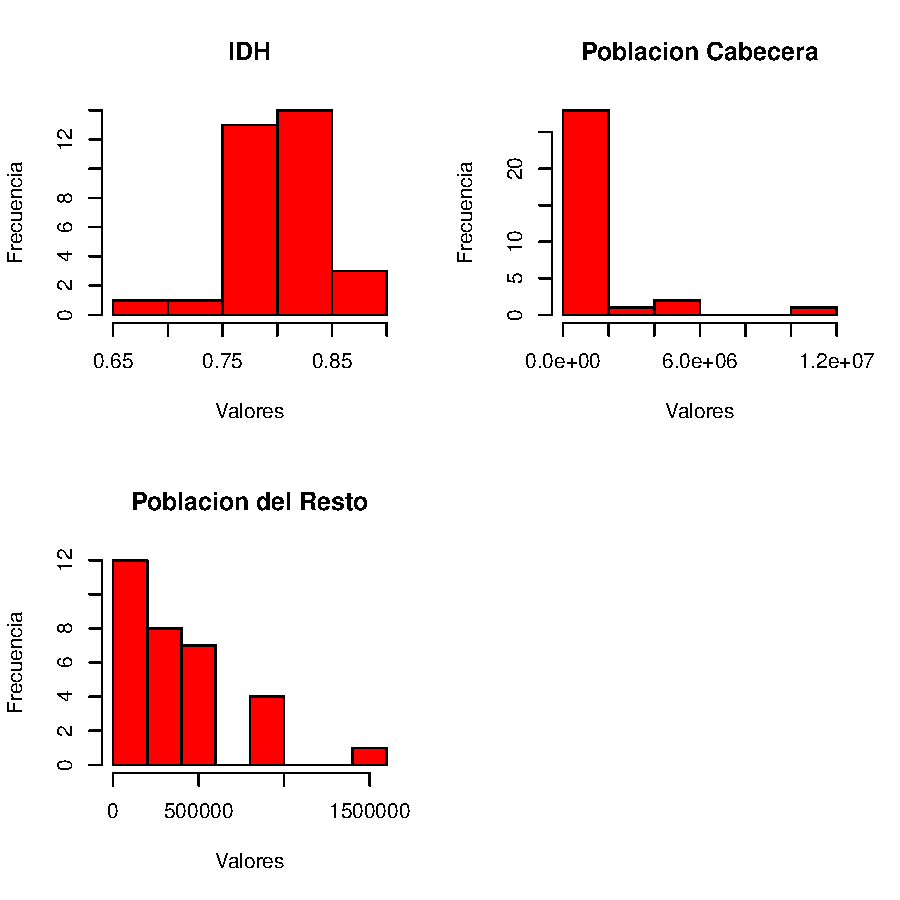
\includegraphics{Preliminar-hist1}
\caption{Distribuci?n de Indicadores}
\label{hist1}
\end{figure}

Si quieren normalizar dado el sesgo de las poblaciones, se tranforma con logaritmo en case 10 y quedaria asi:

\begin{figure}[h]
\centering
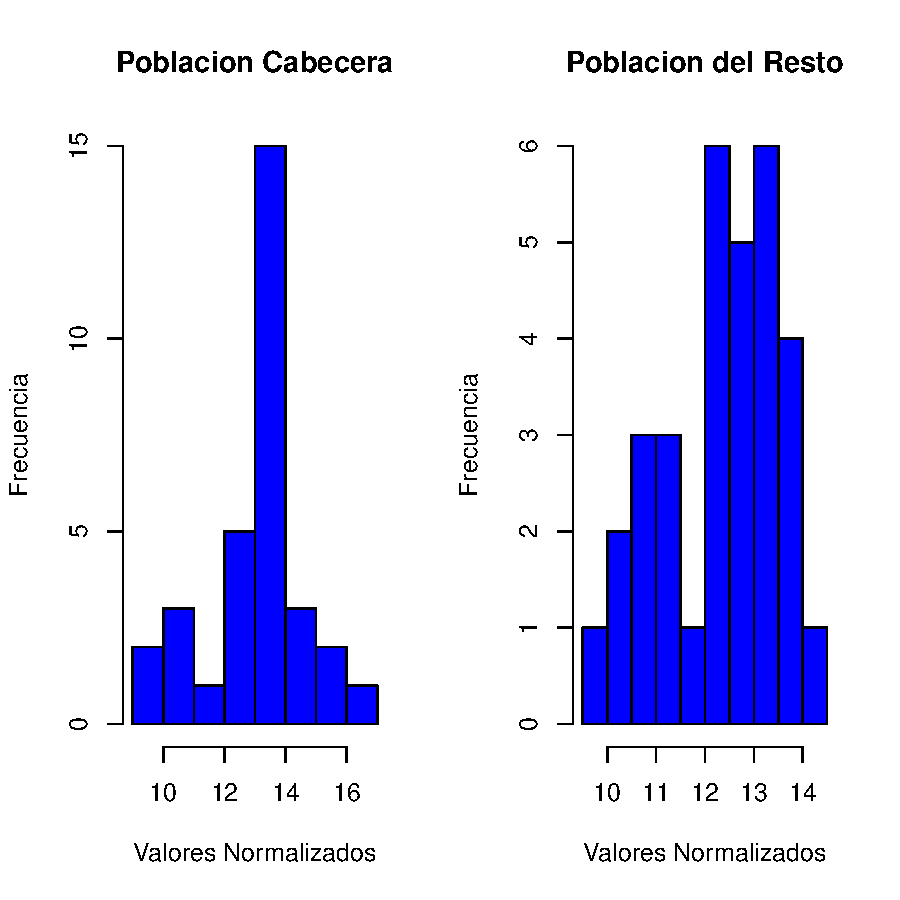
\includegraphics{Preliminar-hist}
\caption{Distribuci?n de Indicadores de Poblaciones Normalizado}
\label{hist}
\end{figure}




\clearpage
%%%%%%%%%%%%%%%%%%%%%%%%%%%%%%%%%%%%%%%%%%%%%%%%%%%%%%%%%%%%%%%%%%%%%%%%%%%%%%%%%%%%%%5
\section{Exploración Bivariada}\label{bivariada}



\begin{Schunk}
\begin{Soutput}
       cabeLog  restoLog
[1,] 0.4873974 0.1773112
\end{Soutput}
\begin{Soutput}
         cabeLog restoLog
cabeLog  "1"     ""      
restoLog "0.84"  "1"     
\end{Soutput}
\end{Schunk}
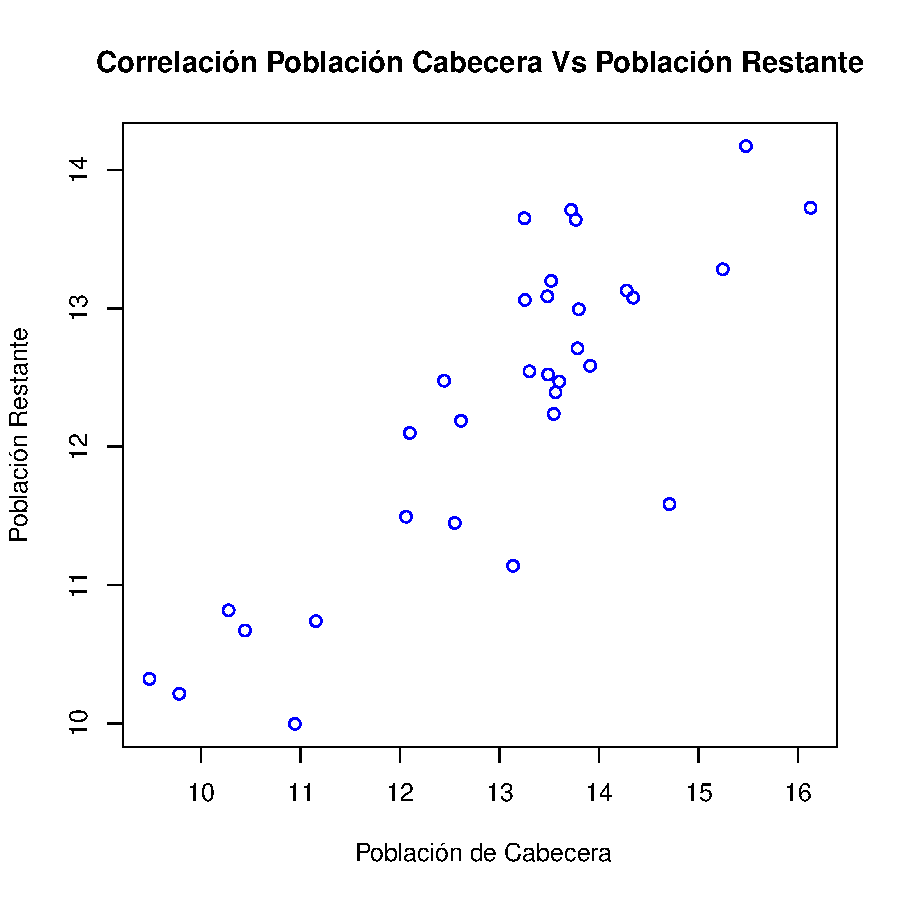
\includegraphics{Preliminar-correl}

\clearpage
%%%%%%%%%%%%%%%%%%%%%%%%%%%%%%%%%%%%%%%%%%%%%%%%%%%%%%%%%%%%%%%%%%%%%%
%%%%%%%%%%%%%%%%Regresion

\section{Modelos de Regresion}

En conclusión, vemos los modelos propuestos. Primero sin la poblacion restante como variable independiente, y luego con está. Los resultados se muestran en la Tabla \ref{regresiones} de la página \pageref{regresiones}.



% Table created by stargazer v.5.2.2 by Marek Hlavac, Harvard University. E-mail: hlavac at fas.harvard.edu
% Date and time: vie., jun. 29, 2018 - 6:42:54 p.m.
\begin{table}[!htbp] \centering 
  \caption{Modelos de Regresión} 
  \label{regresiones} 
\begin{tabular}{@{\extracolsep{5pt}}lcc} 
\\[-1.8ex]\hline 
\hline \\[-1.8ex] 
 & \multicolumn{2}{c}{\textit{Dependent variable:}} \\ 
\cline{2-3} 
\\[-1.8ex] & \multicolumn{2}{c}{IDH} \\ 
\\[-1.8ex] & (1) & (2)\\ 
\hline \\[-1.8ex] 
 cabeLog & 0.013$^{***}$ & 0.031$^{***}$ \\ 
  & (0.004) & (0.007) \\ 
  & & \\ 
 restoLog &  & $-$0.030$^{***}$ \\ 
  &  & (0.010) \\ 
  & & \\ 
 Constant & 0.634$^{***}$ & 0.766$^{***}$ \\ 
  & (0.055) & (0.065) \\ 
  & & \\ 
\hline \\[-1.8ex] 
Observations & 32 & 32 \\ 
R$^{2}$ & 0.238 & 0.425 \\ 
Adjusted R$^{2}$ & 0.212 & 0.385 \\ 
Residual Std. Error & 0.037 (df = 30) & 0.033 (df = 29) \\ 
F Statistic & 9.347$^{***}$ (df = 1; 30) & 10.706$^{***}$ (df = 2; 29) \\ 
\hline 
\hline \\[-1.8ex] 
\textit{Note:}  & \multicolumn{2}{r}{$^{*}$p$<$0.1; $^{**}$p$<$0.05; $^{***}$p$<$0.01} \\ 
\end{tabular} 
\end{table} 




%%%%%%%%%%%%%%%%%%%%%%%%%%%%%%%%%%%%%%%%%%%%%%%%%%%%%%%%%%%%%%%%%%%%%%%


\section{Exploración Espacial}

Como acabamos de ver en la Tabla \ref{regresiones} en la página \pageref{regresiones}, si quisieras sintetizar la multidimensionalidad de nuestros indicadores, podrÃ<U+00AD>amos usar tres de las cuatro variables que tenemos (un par de las originales tiene demasiada correlación). 

AsÃ<U+00AD>, propongo que calculemos conglomerados de paÃ<U+00AD>ses usando toda la información de tres de los indicadores. Como nuestras variables son ordinales utilizaremos un proceso de conglomeración donde las distancia serán calculadas usando la medida {\bf gower} propuestas en \cite{gower_general_1971}, y para los enlazamientos usaremos la técnica de {\bf medoides} según \cite{reynolds_clustering_2006}. Los tres conglomerados se muestran en la Figura \ref{clustmap}.






\begin{figure}[h]
\centering
\begin{Schunk}
\begin{Soutput}
  Group.1       IDH  cabeLog restoLog
1       1 0.7890000 11.42861 11.21085
2       2 0.7944545 13.54188 12.74991
3       3 0.8575000 15.28062 13.57715
\end{Soutput}
\end{Schunk}
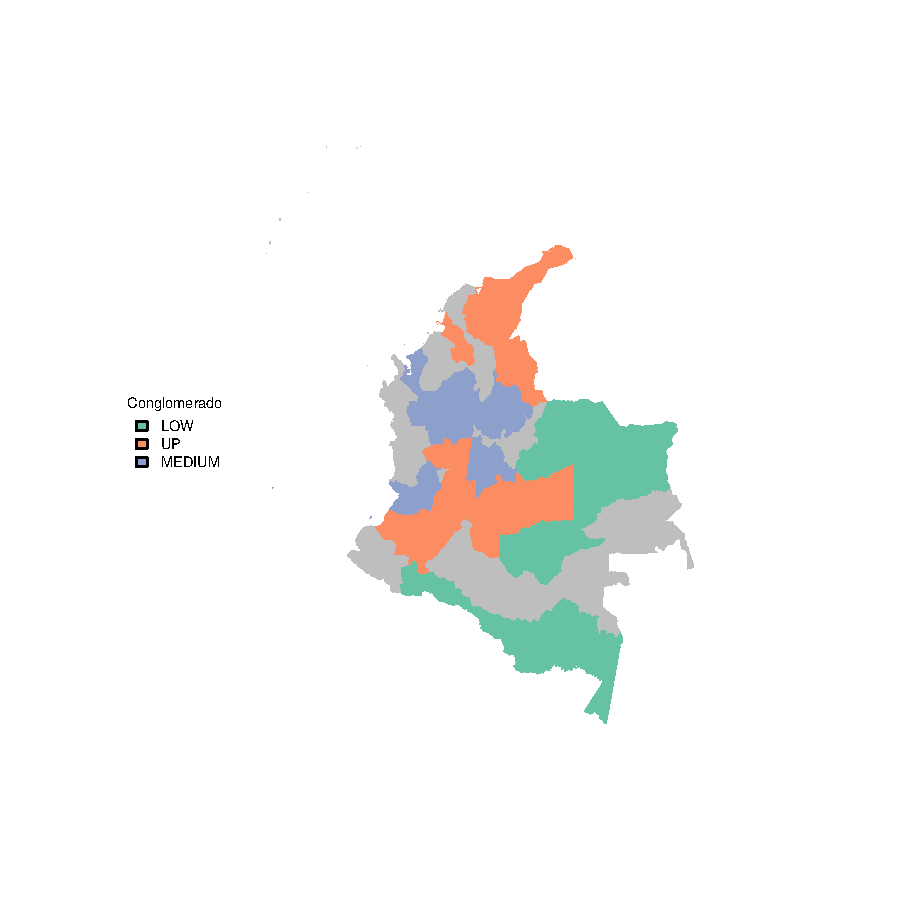
\includegraphics{Preliminar-plotMap1}

\caption{Paises conglomerados segun sus indicadores sociopolÃ<U+00AD>ticos}\label{clustmap}
\end{figure}
%%%%%%%%%%%%%%%%%%%%%%%%%%%%%%%%%%%%%%%%%%%%%%%%%%%





\bibliographystyle{apalike}
\renewcommand{\refname}{Bibliografia}
\bibliography{Bibliografia}
\end{document}
